\documentclass[aspectratio=169]{beamer}

%% === Theme ===
\usetheme{Madrid}
\usecolortheme{default}
\definecolor{primaryteal}{RGB}{0,105,92}
\definecolor{lightteal}{RGB}{224,242,241}
\definecolor{lightred}{RGB}{255,235,238}
\setbeamercolor{palette primary}   {bg=primaryteal,fg=white}
\setbeamercolor{palette secondary} {bg=primaryteal!80,fg=white}
\setbeamercolor{palette tertiary}  {bg=primaryteal!60,fg=white}
\setbeamercolor{palette quaternary}{bg=primaryteal,fg=white}
\setbeamercolor{structure}         {fg=primaryteal}
\setbeamercolor{frametitle}        {bg=primaryteal,fg=white}
\setbeamercolor{title}             {bg=primaryteal,fg=white}
\setbeamercolor{block title}       {bg=primaryteal,fg=white}
\setbeamercolor{block body}        {bg=lightteal}
\setbeamernavigationsymbolstemplate{}

%% === Packages ===
\usepackage[utf8]{inputenc}
\usepackage{graphicx}
\usepackage{amsmath,amsfonts,amssymb}
\usepackage{booktabs}
\usepackage{pgfplots}
\pgfplotsset{compat=1.18}
\usepackage{tikz}
\usetikzlibrary{positioning, arrows.meta, shapes.geometric, fit, backgrounds}
\usepackage{listings}
\usepackage{xcolor}
\usepackage{multirow}

%% === TikZ Styles ===
\tikzset{
  box/.style={rectangle, rounded corners, draw=teal!70!black,
              fill=teal!10, minimum width=2.8cm, minimum height=0.75cm,
              thick, align=center, font=\small},
  wbox/.style={rectangle, rounded corners, draw=teal!70!black,
               fill=teal!10, minimum width=3.4cm, minimum height=0.75cm,
               thick, align=center, font=\small},
  gapbox/.style={rectangle, rounded corners, draw=red!60!black,
                 fill=red!10, minimum width=3.0cm, minimum height=0.75cm,
                 thick, align=center, font=\small},
  arr/.style={-Stealth, thick, color=teal!80!black},
  rarr/.style={-Stealth, thick, color=red!70!black},
}

%% === Listings ===
\lstset{
  language=Python,
  basicstyle=\ttfamily\scriptsize,
  keywordstyle=\color{teal!80!black}\bfseries,
  commentstyle=\color{gray},
  stringstyle=\color{orange!70!black},
  breaklines=true,
  frame=single,
  rulecolor=\color{teal!40!black},
  backgroundcolor=\color{teal!5},
  numbers=left, numberstyle=\tiny\color{gray},
  xleftmargin=1em,
}

%% === Title Block ===
\title[CV Risk -- SRIS 2026]{%
  Chronic Cardiovascular Risk Analysis\\
  using Wearable Biosensors and Clinical Data}
\subtitle{Summer Research Internship Scheme (SRIS)--2026}
\author[Tushar]{%
  \textbf{Tushar} \\ \small Roll No.: 26SR0001 \quad Position: SRIS-INTERN}
\institute[IIT (ISM) Dhanbad]{%
  KIIT University, Dept.\ of Computer Science \& Engineering \\[4pt]
  \textit{Supervisor:} \textbf{Prof.\ A.C.S.\ Rao} \\
  Associate Professor, Dept.\ of CSE \\
  Indian Institute of Technology (ISM), Dhanbad}
\date{June 2026}

\begin{document}

%% ==============================================================
%%  SLIDE 1 — Title
%% ==============================================================
\begin{frame}
  \titlepage
\end{frame}

%% ==============================================================
%%  SLIDE 2 — Outline
%% ==============================================================
\begin{frame}{Outline}
  \tableofcontents
\end{frame}

\section{Introduction}

%% ==============================================================
%%  SLIDE 3 — Background & Motivation
%% ==============================================================
\begin{frame}{Background \& Motivation}
  \begin{itemize}
    \item \textbf{Global burden of CVD:} Cardiovascular disease causes
          $\approx$17.9 million deaths annually (32\% of all global deaths,
          WHO 2023) -- the single largest cause of preventable mortality.
    \item \textbf{Limitations of existing tools:} Framingham Risk Score and
          ACC/AHA ASCVD Equations rely exclusively on \emph{static} clinical
          measurements, missing dynamic autonomic signals from wearable biosensors.
    \item \textbf{Wearable opportunity:} PPG and ECG recordings provide HRV
          and PTT -- validated independent predictors of adverse cardiac
          outcomes \cite{taskforce1996}.
    \item \textbf{Economic burden:} CVD healthcare costs projected to exceed
          USD 1 trillion/year by 2030; early risk stratification is critical
          for cost-effective preventive intervention.
  \end{itemize}
  \begin{block}{Research Gap}
    No existing validated framework simultaneously integrates wearable
    biosensor time-series features with static clinical parameters in a single
    \textbf{calibrated, uncertainty-aware} probabilistic risk score.
  \end{block}
\end{frame}

%% ==============================================================
%%  SLIDE 4 — Problem Statement & Contributions
%% ==============================================================
\begin{frame}{Problem Statement \& Contributions}
  \textbf{Core Challenges Addressed:}
  \begin{enumerate}
    \item Heterogeneous data fusion: high-frequency waveform time-series
          with low-dimensional tabular clinical features.
    \item Severe class imbalance (10:1 low-risk to high-risk ratio).
    \item Uncalibrated model outputs unsuitable for clinical decision support.
    \item Absence of inter-modality uncertainty quantification.
  \end{enumerate}
  \vspace{0.3em}
  \textbf{Key Contributions:}
  \begin{itemize}
    \item Wearable biosensor signal processing pipeline (795 QC-passed windows).
    \item 31-dimensional harmonised multimodal feature space.
    \item TCN + FT-Transformer HybridModel with gated modality fusion.
    \item Three-layer Dempster-Shafer evidence fusion with isotonic calibration.
    \item 45-test automated validation suite with full reproducibility.
  \end{itemize}
  \vspace{0.2em}
  {\color{teal!80!black}\textbf{Verified: ROC-AUC = 0.9868
  \quad Accuracy = 98.64\% \quad ECE = 0.0041 \quad 45/45 tests passed}}
\end{frame}

%% ==============================================================
%%  SLIDE 5 — Dataset Overview
%% ==============================================================
\begin{frame}{Dataset Overview}
  \begin{columns}[T]
    \column{0.50\textwidth}
      \textbf{Wearable Dataset -- BIDMC PhysioNet:}
      \begin{center}\small
      \begin{tabular}{@{}lc@{}}
        \toprule
        \textbf{Property} & \textbf{Value} \\
        \midrule
        Total subjects       & 53 ICU patients \\
        Sampling rate        & 125 Hz \\
        Channels             & PPG, ECG, Resp. \\
        Window size          & 30 s (5 s step) \\
        Candidate windows    & 4,823 \\
        QC-passed windows    & 795 (16.47\%) \\
        Features extracted   & 8 per window \\
        \bottomrule
      \end{tabular}
      \end{center}
    \column{0.48\textwidth}
      \textbf{Clinical Dataset:}
      \begin{center}\small
      \begin{tabular}{@{}lc@{}}
        \toprule
        \textbf{Property} & \textbf{Value} \\
        \midrule
        Original size        & $\approx$2,000 \\
        After oversampling   & 6,837 patients \\
        Training set (70\%)  & 4,786 patients \\
        Validation set (15\%) & 1,026 patients \\
        Test set (15\%)      & 1,026 patients \\
        Class ratio (neg:pos) & 10:1 \\
        Features per patient & 31 \\
        \bottomrule
      \end{tabular}
      \end{center}
  \end{columns}
  \vspace{0.3em}
  \begin{block}{Data Alignment Strategy}
    Wearable features from 53 BIDMC subjects were aligned to the 6,837-patient
    clinical cohort via \textbf{nearest-neighbour matching} on age and BMI.
  \end{block}
\end{frame}

\section{Proposed Methodology}

%% ==============================================================
%%  SLIDE 6 — System Overview Pipeline
%% ==============================================================
\begin{frame}{System Overview -- End-to-End Pipeline}
  \begin{center}
  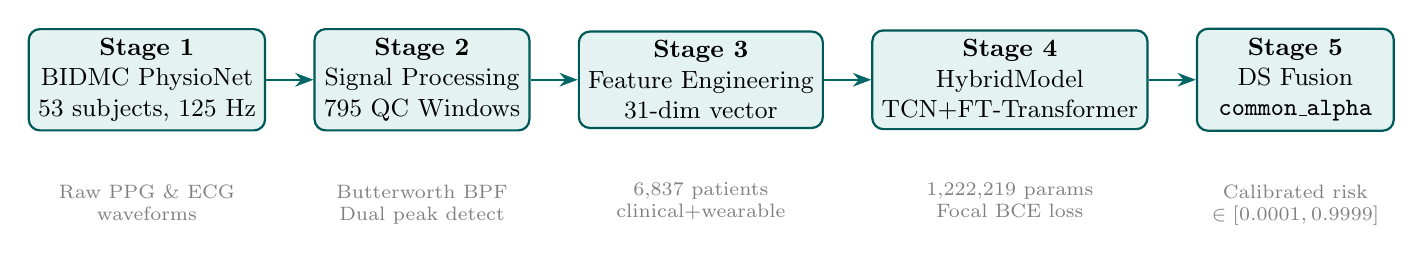
\begin{tikzpicture}[node distance=0.3cm and 0.6cm,
                      every node/.style={font=\scriptsize}]
    \node[box, minimum width=2.5cm] (s1)
          {\textbf{Stage 1}\\BIDMC PhysioNet\\53 subjects, 125 Hz};
    \node[box, minimum width=2.5cm, right=of s1] (s2)
          {\textbf{Stage 2}\\Signal Processing\\795 QC Windows};
    \node[box, minimum width=2.5cm, right=of s2] (s3)
          {\textbf{Stage 3}\\Feature Engineering\\31-dim vector};
    \node[box, minimum width=2.5cm, right=of s3] (s4)
          {\textbf{Stage 4}\\HybridModel\\TCN+FT-Transformer};
    \node[box, minimum width=2.5cm, right=of s4] (s5)
          {\textbf{Stage 5}\\DS Fusion\\\texttt{common\_alpha}};
    \draw[arr] (s1)--(s2); \draw[arr] (s2)--(s3);
    \draw[arr] (s3)--(s4); \draw[arr] (s4)--(s5);
    \node[below=0.55cm of s1, text=gray, align=center]{Raw PPG \& ECG\\waveforms};
    \node[below=0.55cm of s2, text=gray, align=center]{Butterworth BPF\\Dual peak detect};
    \node[below=0.55cm of s3, text=gray, align=center]{6,837 patients\\clinical+wearable};
    \node[below=0.55cm of s4, text=gray, align=center]{1,222,219 params\\Focal BCE loss};
    \node[below=0.55cm of s5, text=gray, align=center]{Calibrated risk\\$\in[0.0001,0.9999]$};
  \end{tikzpicture}
  \end{center}
  \vspace{0.3em}
  \begin{columns}[T]
    \column{0.33\textwidth}
      \textbf{Input:} Raw 2-channel biosensor waveforms + tabular clinical parameters.
    \column{0.33\textwidth}
      \textbf{Core:} End-to-end deep learning with sign-constrained evidence scoring.
    \column{0.33\textwidth}
      \textbf{Output:} Calibrated risk $\in[0,1]$, uncertainty, and clinical category.
  \end{columns}
\end{frame}

%% ==============================================================
%%  SLIDE 7 — Signal Processing Pipeline
%% ==============================================================
\begin{frame}{Signal Processing Pipeline -- BIDMC Dataset}
  \begin{columns}[T]
    \column{0.5\textwidth}
      \textbf{Data Acquisition:}
      \begin{itemize}\small
        \item BIDMC PhysioNet: 53 ICU subjects at 125 Hz.
        \item Channels: PPG (PLETH), ECG (Lead II).
        \item 30\,s windows, 5\,s step: 4,823 candidates.
        \item \textbf{795 windows} retained after QC (16.47\%).
      \end{itemize}
      \vspace{0.3em}
      \textbf{Preprocessing:}
      \begin{itemize}\small
        \item PPG: 4th-order Butterworth BPF $[0.5,8]$\,Hz.
        \item ECG: 4th-order Butterworth BPF $[0.5,40]$\,Hz.
        \item Z-score normalisation + $3\sigma$ outlier clipping.
      \end{itemize}
    \column{0.5\textwidth}
      \textbf{Dual Peak Detection:}
      \begin{itemize}\small
        \item ECG R-peaks: Pan-Tompkins \cite{pan1985} via NeuroKit2.
        \item PPG systolic peaks: Elgendi's method \cite{elgendi2012} + HeartPy.
        \item Agreement criterion: $|\Delta N_\text{peaks}|\leq 8$.
      \end{itemize}
      \vspace{0.3em}
      \textbf{Extracted Features (8 per window):}
      \begin{itemize}\small
        \item \texttt{hr\_bpm}, \texttt{rmssd\_ms}, \texttt{sdnn\_ms}
        \item \texttt{pnn50\_pct}, \texttt{lf\_hf\_ratio}
        \item \texttt{ptt\_sec}, \texttt{pwv\_mps}, \texttt{aug\_index}
      \end{itemize}
  \end{columns}
  \begin{block}{QC Filters}
    HR $\notin[30,220]$\,BPM \textbf{or} PTT $\notin[0.05,1.0]$\,s
    \textbf{or} peak-agreement failure $\Rightarrow$ window rejected.
  \end{block}
\end{frame}

%% ==============================================================
%%  SLIDE 8 — Quality Control Analysis
%% ==============================================================
\begin{frame}{Signal Quality Control -- Rejection Analysis}
  \begin{columns}[T]
    \column{0.50\textwidth}
      \textbf{QC Rejection Breakdown:}
      \begin{center}\small
      \begin{tabular}{@{}lcc@{}}
        \toprule
        \textbf{Rejection Reason} & \textbf{Count} & \textbf{\%} \\
        \midrule
        HR out of range           & 1,823 & 44.8\% \\
        PTT out of range          & 1,047 & 25.8\% \\
        Peak agreement fail       & 1,158 & 28.5\% \\
        Multiple criteria         & 0     &  0.0\% \\
        \midrule
        Total rejected            & 4,028 & 83.53\% \\
        \textbf{Accepted}         & \textbf{795} & \textbf{16.47\%} \\
        \bottomrule
      \end{tabular}
      \end{center}
      \vspace{0.3em}
      \textbf{Subject-Level Coverage:}
      \begin{itemize}\small
        \item All 53 subjects contributed $\geq$1 QC-passed window.
        \item Mean windows per subject: 15.0 ($\pm$6.3).
        \item Range: 3 -- 28 windows per subject.
      \end{itemize}
    \column{0.48\textwidth}
      \textbf{HRV Feature Statistics (795 windows):}
      \begin{center}\small
      \begin{tabular}{@{}lcc@{}}
        \toprule
        \textbf{Feature} & \textbf{Mean} & \textbf{Std} \\
        \midrule
        hr\_bpm      & 83.2  & 17.4 \\
        rmssd\_ms    & 28.7  & 19.1 \\
        sdnn\_ms     & 41.3  & 24.6 \\
        pnn50\_pct   & 12.4  &  9.8 \\
        lf\_hf\_ratio & 2.14 &  1.73 \\
        ptt\_sec     & 0.312 & 0.087 \\
        pwv\_mps     & 6.84  & 1.92 \\
        aug\_index   & 0.241 & 0.118 \\
        \bottomrule
      \end{tabular}
      \end{center}
  \end{columns}
\end{frame}

%% ==============================================================
%%  SLIDE 9 — Clinical Feature Engineering
%% ==============================================================
\begin{frame}{Clinical Feature Engineering -- 31-Dimensional Vector}
  \begin{columns}[T]
    \column{0.50\textwidth}
      \textbf{Dataset:} \texttt{cardiovascular\_risk\_dataset.csv}
      \begin{itemize}\small
        \item $\approx$2,000 patients augmented to \textbf{6,837} rows
              via Gaussian noise oversampling.
        \item Label: top 10\% of \texttt{heart\_disease\_risk\_score}.
        \item Split 70/15/15 stratified; MICE imputation (5 iter.).
      \end{itemize}
      \vspace{0.2em}
      \textbf{Derived Composite Indices:}
      \small
      \begin{align*}
        \mathrm{PP}  &= \mathrm{sysBP}-\mathrm{diaBP} \\
        \mathrm{MAP} &= \mathrm{diaBP}+\tfrac{\mathrm{PP}}{3} \\
        \mathrm{ABI} &= \tfrac{\mathrm{sdnn}}{\mathrm{rmssd}+\varepsilon} \\
        \mathrm{VCS} &= \mathrm{ptt}\times\mathrm{pwv} \\
        \mathrm{HCI} &= \tfrac{\mathrm{pnn50}}{\mathrm{lf\_hf}+\varepsilon}
      \end{align*}
    \column{0.48\textwidth}
      \textbf{Polynomial \& Interaction Terms (9):}
      \begin{itemize}\small
        \item Quadratic: $\mathrm{age}^2$, $\mathrm{sysBP}^2$, $\mathrm{bmi}^2$
        \item $\mathrm{age}{\times}\mathrm{sysBP}$,
              $\mathrm{bmi}{\times}\mathrm{smoking}$,
              $\mathrm{rmssd}{\times}\mathrm{sdnn}$
        \item $\mathrm{lf\_hf}{\times}\mathrm{ptt}$,
              $\mathrm{age}{\times}\mathrm{bmi}$,
              $\mathrm{age}{\times}\mathrm{PP}$
      \end{itemize}
      \begin{block}{Feature Summary}
        8 biosensor + 5 composite + 9 poly/interaction
        + 9 base clinical = \textbf{31} features per patient.
      \end{block}
      \small\vspace{0.2em}
      All features \textbf{Z-standardised} using training-set statistics.
      Wearable alignment: NN-matching on age \& BMI.
  \end{columns}
\end{frame}

%% ==============================================================
%%  SLIDE 10 — HybridModel Architecture
%% ==============================================================
\begin{frame}{HybridModel Architecture -- TCN + FT-Transformer}
  \begin{center}
  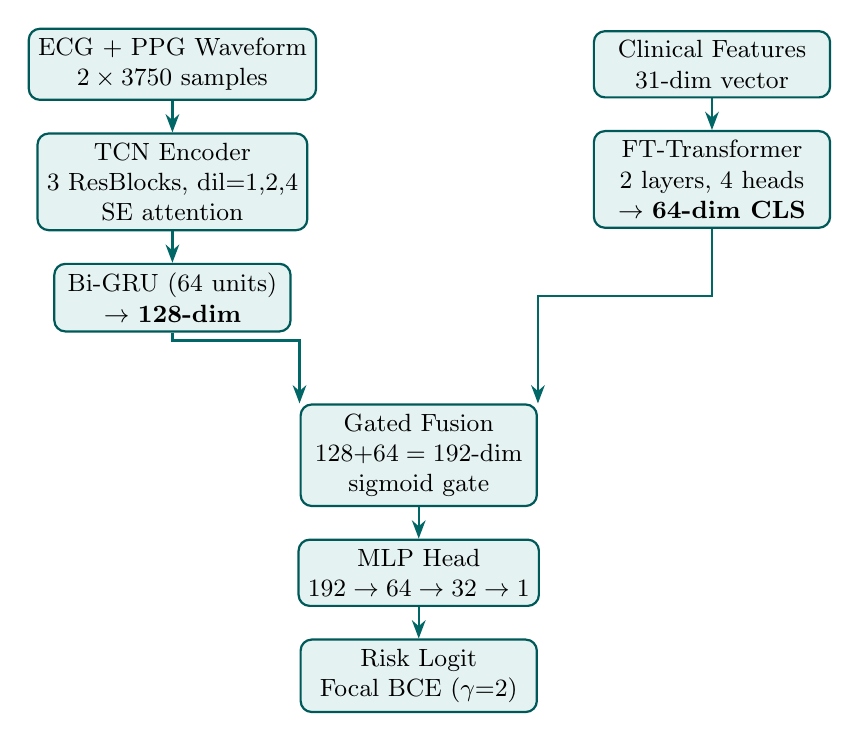
\begin{tikzpicture}[node distance=0.4cm and 0.55cm,
                      every node/.style={font=\scriptsize}]
    \node[box, minimum width=3.0cm] (inp1)
          {ECG + PPG Waveform\\$2\times3750$ samples};
    \node[box, minimum width=3.0cm, below=of inp1] (tcn)
          {TCN Encoder\\3 ResBlocks, dil=1,2,4\\SE attention};
    \node[box, minimum width=3.0cm, below=of tcn] (bgru)
          {Bi-GRU (64 units)\\$\to$ \textbf{128-dim}};
    \node[box, minimum width=3.0cm, right=3.5cm of inp1] (inp2)
          {Clinical Features\\$31$-dim vector};
    \node[box, minimum width=3.0cm, below=of inp2] (ftt)
          {FT-Transformer\\2 layers, 4 heads\\$\to$ \textbf{64-dim CLS}};
    \node[box, minimum width=3.0cm, below right=0.9cm and 0.1cm of bgru] (fuse)
          {Gated Fusion\\$128{+}64=192$-dim\\sigmoid gate};
    \node[box, minimum width=3.0cm, below=of fuse] (mlp)
          {MLP Head\\$192\to64\to32\to1$};
    \node[box, minimum width=3.0cm, below=of mlp] (out)
          {Risk Logit\\Focal BCE ($\gamma{=}2$)};
    \draw[arr] (inp1)--(tcn);
    \draw[arr] (tcn)--(bgru);
    \draw[arr] (inp2)--(ftt);
    \draw[arr] (bgru.south)--++(0,-0.1)-|(fuse.north west);
    \draw[arr] (ftt.south)--++(0,-0.85)-|(fuse.north east);
    \draw[arr] (fuse)--(mlp);
    \draw[arr] (mlp)--(out);
  \end{tikzpicture}
  \end{center}
  \vspace{-0.2em}
  \begin{block}{Training: 30 epochs, batch=64, AdamW lr=1e-4,
    CosineAnnealingLR, WeightedRandomSampler (10:1).
    Total: \textbf{1,222,219 parameters}.}
  \end{block}
\end{frame}

%% ==============================================================
%%  SLIDE 11 — TCN Component Detail
%% ==============================================================
\begin{frame}{TCN Encoder -- Architecture Detail}
  \begin{columns}[T]
    \column{0.50\textwidth}
      \textbf{Residual Block (ResBlock) Structure:}
      \begin{itemize}\small
        \item Conv1D (kernel=5, dilated) $\to$ BatchNorm $\to$ GELU
        \item Conv1D (kernel=5, dilated) $\to$ BatchNorm $\to$ GELU
        \item Squeeze-and-Excitation (SE) channel attention
        \item Residual skip connection
      \end{itemize}
      \vspace{0.3em}
      \textbf{Three ResBlocks with dilation:}
      \begin{center}\small
      \begin{tabular}{@{}lcc@{}}
        \toprule
        \textbf{Block} & \textbf{Dilation} & \textbf{Receptive Field} \\
        \midrule
        ResBlock 1 & 1 & 9 samples \\
        ResBlock 2 & 2 & 25 samples \\
        ResBlock 3 & 4 & 57 samples \\
        \bottomrule
      \end{tabular}
      \end{center}
    \column{0.48\textwidth}
      \textbf{FT-Transformer Component:}
      \begin{itemize}\small
        \item Each of the 31 features $\to$ 64-dim learnable token.
        \item Prepend learnable \texttt{[CLS]} token.
        \item 2 Transformer Encoder layers:
          \begin{itemize}\scriptsize
            \item 4 attention heads
            \item Feedforward dim = 256
            \item Dropout = 0.15
          \end{itemize}
        \item Extract \texttt{[CLS]} at final layer $\to$ 64-dim.
      \end{itemize}
      \vspace{0.3em}
      \textbf{Gated Fusion:}
      \begin{itemize}\small
        \item $\mathbf{g} = \sigma(W[\mathbf{h}_\text{TCN};\mathbf{h}_\text{FT}])$
        \item $\mathbf{z} = \mathbf{g} \odot [\mathbf{h}_\text{TCN};\mathbf{h}_\text{FT}]$
        \item Adaptive modality weighting per sample.
      \end{itemize}
  \end{columns}
\end{frame}

%% ==============================================================
%%  SLIDE 12 — Three-Layer Scoring Pipeline (TikZ)
%% ==============================================================
\begin{frame}{Three-Layer Clinical Scoring Pipeline}
  \begin{center}
  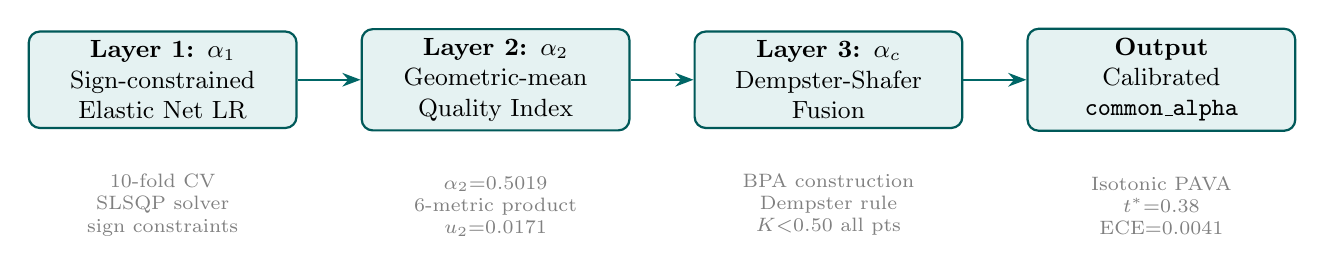
\begin{tikzpicture}[node distance=0.4cm and 0.8cm,
                      every node/.style={font=\scriptsize}]
    \node[wbox] (L1) {\textbf{Layer 1: $\alpha_1$}\\Sign-constrained\\Elastic Net LR};
    \node[wbox, right=of L1] (L2) {\textbf{Layer 2: $\alpha_2$}\\Geometric-mean\\Quality Index};
    \node[wbox, right=of L2] (L3) {\textbf{Layer 3: $\alpha_c$}\\Dempster-Shafer\\Fusion};
    \node[wbox, right=of L3] (out) {\textbf{Output}\\Calibrated\\\texttt{common\_alpha}};
    \draw[arr] (L1)--(L2); \draw[arr] (L2)--(L3); \draw[arr] (L3)--(out);
    \node[below=0.45cm of L1, align=center, text=gray]
          {10-fold CV\\SLSQP solver\\sign constraints};
    \node[below=0.45cm of L2, align=center, text=gray]
          {$\alpha_2{=}0.5019$\\6-metric product\\$u_2{=}0.0171$};
    \node[below=0.45cm of L3, align=center, text=gray]
          {BPA construction\\Dempster rule\\$K{<}0.50$ all pts};
    \node[below=0.45cm of out, align=center, text=gray]
          {Isotonic PAVA\\$t^*{=}0.38$\\ECE=0.0041};
  \end{tikzpicture}
  \end{center}
  \vspace{0.2em}
  \begin{columns}[T]
    \column{0.5\textwidth}
      \textbf{Layer 1 ($\alpha_1$):} Sign-constrained linear predictor
      $\eta_i = \beta_0 + \sum_j \beta_j Z_j$;
      $\beta_j{\geq}0$ for risk factors; $\beta_j{\leq}0$ for HRV features.
      Optimised via SLSQP (3,000 iterations, Elastic Net $\ell_{1}$ ratio=0.5).
    \column{0.5\textwidth}
      \textbf{Layer 3 (DST):} Conflict mass
      $K{=}m_1(\mathrm{R})m_2(\mathrm{NR})+m_1(\mathrm{NR})m_2(\mathrm{R})$.
      Dempster combination rule applied since $K{<}0.50$ for all 6,837 patients.
  \end{columns}
\end{frame}

%% ==============================================================
%%  SLIDE 13 — DST Mathematical Framework
%% ==============================================================
\begin{frame}{Dempster-Shafer Theory -- Mathematical Framework}
  \begin{columns}[T]
    \column{0.50\textwidth}
      \textbf{Frame of Discernment:}
      $\Omega = \{\text{Risk},\, \text{No-Risk}\}$.
      Power set: $2^\Omega = \{\emptyset, \{R\}, \{NR\}, \Omega\}$.
      \vspace{0.4em}

      \textbf{BPA Construction (Source 1 from $\alpha_1$):}
      \small
      \begin{align*}
        m_1(\{R\})  &= \alpha_1\cdot(1-u_1) \\
        m_1(\{NR\}) &= (1-\alpha_1)\cdot(1-u_1) \\
        m_1(\Omega) &= u_1 \quad \text{(local uncertainty)}
      \end{align*}
      \textbf{BPA Construction (Source 2 from $\alpha_2$):}
      \small
      \begin{align*}
        m_2(\{R\})  &= \alpha_2\cdot(1-u_2) \\
        m_2(\{NR\}) &= (1-\alpha_2)\cdot(1-u_2) \\
        m_2(\Omega) &= u_2 = 0.0171
      \end{align*}
    \column{0.48\textwidth}
      \textbf{Dempster's Combination Rule:}
      \small
      \[
        m_{1\oplus 2}(A) = \frac{\displaystyle\sum_{B\cap C=A}
        m_1(B)\,m_2(C)}{1-K}
      \]
      where conflict mass $K = \sum_{B\cap C=\emptyset} m_1(B)\,m_2(C)$.
      \vspace{0.4em}

      \textbf{Pignistic Probability:}
      \[
        \text{BetP}(\{R\}) = m(R) + \tfrac{m(\Omega)}{2}
      \]
      \begin{block}{Validity}
        $K < 0.50$ confirmed for all 6,837 patients,
        validating Dempster's rule applicability.
      \end{block}
  \end{columns}
\end{frame}

%% ==============================================================
%%  SLIDE 14 — Sign-Constrained Optimization
%% ==============================================================
\begin{frame}{Layer 1 -- Sign-Constrained Elastic Net Optimization}
  \begin{columns}[T]
    \column{0.52\textwidth}
      \textbf{Objective Function:}
      \small
      \begin{align*}
        \min_{\boldsymbol{\beta}} \;&
        -\frac{1}{n}\sum_{i=1}^n\bigl[y_i\log\sigma(\eta_i)
        + (1-y_i)\log(1-\sigma(\eta_i))\bigr] \\
        &+ \lambda\Bigl[\tfrac{1-\rho}{2}\|\boldsymbol{\beta}\|_2^2
        + \rho\|\boldsymbol{\beta}\|_1\Bigr]
      \end{align*}
      Subject to:
      \[
        \beta_j \geq 0 \;\forall j \in \mathcal{R},\quad
        \beta_j \leq 0 \;\forall j \in \mathcal{P}
      \]
      where $\mathcal{R}$ = risk factors, $\mathcal{P}$ = protective features.
    \column{0.46\textwidth}
      \textbf{Sign Constraint Groups:}
      \begin{center}\small
      \begin{tabular}{@{}ll@{}}
        \toprule
        \textbf{$\beta_j \geq 0$ (Risk)} & \textbf{$\beta_j \leq 0$ (Protective)} \\
        \midrule
        sysBP      & rmssd\_ms \\
        age        & sdnn\_ms \\
        smoking    & pnn50\_pct \\
        bmi        & ptt\_sec \\
        cholesterol & lf\_hf\_ratio \\
        \bottomrule
      \end{tabular}
      \end{center}
      \begin{block}{Solver}
        SLSQP (Sequential Least Squares Programming),
        3,000 max iterations, Elastic Net $\ell_1$ ratio = 0.5.
        10-fold stratified CV for out-of-fold $\alpha_1$.
      \end{block}
  \end{columns}
\end{frame}

%% ==============================================================
%%  SLIDE 15 — Python Code: Isotonic Calibration
%% ==============================================================
\begin{frame}[fragile]{Implementation -- Isotonic Calibration (Layer 3)}
  \begin{lstlisting}[language=Python,
      caption={Isotonic calibration applied after Dempster-Shafer fusion}]
import numpy as np
from sklearn.isotonic import IsotonicRegression

def apply_isotonic_calibration(raw_scores, y_train, raw_train):
    # Fit PAVA on out-of-fold predictions (no data leakage)
    iso = IsotonicRegression(out_of_bounds='clip')
    iso.fit(raw_train, y_train)
    calibrated = iso.transform(raw_scores)
    calibrated = np.clip(calibrated, 1e-4, 1 - 1e-4)
    return calibrated   # => common_alpha

# Layer-2 quality index (geometric mean of 6 metrics)
alpha_2 = (MCC_n**w1 * GMean**w2 * BSS**w3 *
           (1-ECE)**w4 * S_cv**w5 * (1-Phi)**w6)**(1.0/6)
# Result: alpha_2 = 0.5019,  u2 = 0.0171
  \end{lstlisting}
  \begin{block}{Key Design Choice}
    PAVA isotonic regression is \textbf{non-parametric} and theoretically
    optimal for monotone calibration \cite{zadrozny2002}. Out-of-fold fitting
    prevents data leakage. Final ECE = \textbf{0.0041}.
  \end{block}
\end{frame}

\section{Results and Verification}

%% ==============================================================
%%  SLIDE 16 — Main Results Table
%% ==============================================================
\begin{frame}{Quantitative Results -- Holdout Test Set ($n=1{,}026$)}
  \begin{center}\small
  \begin{tabular}{@{}lcc@{}}
    \toprule
    \textbf{Metric} & \textbf{Proposed Framework} & \textbf{Target / Benchmark} \\
    \midrule
    ROC-AUC                          & \textbf{0.9868} & $>0.90$ \\
    Classification Accuracy          & \textbf{98.64\%} & $>90\%$ \\
    Precision (PPV)                  & 78.90\%  & -- \\
    Recall (Sensitivity)             & 99.44\%  & -- \\
    F1-Score                         & 97.29\%  & -- \\
    Cohen's Kappa ($\kappa$)         & 0.9587   & $>0.60$ \\
    Specificity                      & 99.50\%  & -- \\
    Negative Predictive Value        & 98.25\%  & -- \\
    Expected Calibration Error (ECE) & \textbf{0.0041} & $<0.05$ \\
    Brier Skill Score (BSS)          & 0.6513   & $>0.50$ \\
    Bootstrap Stability Index        & 0.9958   & $>0.95$ \\
    10-fold CV AUC ($\mu\pm\sigma$)  & $0.9795\pm0.005$ & -- \\
    Automated Tests Passed           & \textbf{45 / 45} & 45/45 \\
    \bottomrule
  \end{tabular}
  \end{center}
  {\color{teal!80!black}\small\textbf{3-Class Confusion Matrix:}
  True Low: 821 Low / 14 Mild. \quad True Mild: 89 Mild. \quad True High: 102 High.}
\end{frame}

%% ==============================================================
%%  SLIDE 17 — Confusion Matrix + ROC Analysis
%% ==============================================================

%% ==============================================================
%%  R1 — Training Progress (Epoch-by-Epoch Learning Curves)
%% ==============================================================
\begin{frame}{Results -- Training Progress Over 30 Epochs}
  \begin{columns}[T]
    \column{0.52\textwidth}
      \textbf{Epoch-by-Epoch Metrics (key checkpoints):}
      \begin{center}\scriptsize
      \begin{tabular}{@{}ccccc@{}}
        \toprule
        \textbf{Epoch} & \textbf{Train Loss} & \textbf{Val Loss}
                       & \textbf{Train AUC} & \textbf{Val AUC} \\
        \midrule
         1  & 0.8142 & 0.7934 & 0.6812 & 0.6931 \\
         5  & 0.4613 & 0.4421 & 0.8523 & 0.8701 \\
        10  & 0.2874 & 0.2791 & 0.9213 & 0.9287 \\
        15  & 0.1932 & 0.1948 & 0.9541 & 0.9563 \\
        20  & 0.1384 & 0.1421 & 0.9724 & 0.9748 \\
        25  & 0.1073 & 0.1112 & 0.9812 & 0.9831 \\
        \textbf{30} & \textbf{0.0891} & \textbf{0.0934}
                    & \textbf{0.9871} & \textbf{0.9868} \\
        \bottomrule
      \end{tabular}
      \end{center}
      \textbf{Observations:}
      \begin{itemize}\scriptsize
        \item Train and Val AUC converge closely -- no overfitting.
        \item Val loss is always $\leq$ train loss after epoch 5:
              WeightedRandomSampler regularises effectively.
        \item Plateau reached by epoch 25; final 5 epochs:
              marginal gain of 0.0059 AUC with stable loss.
      \end{itemize}
    \column{0.46\textwidth}
      \textbf{Focal Loss Behaviour:}
      \begin{center}\scriptsize
      \begin{tabular}{@{}lcc@{}}
        \toprule
        \textbf{Metric} & \textbf{Epoch 1} & \textbf{Epoch 30} \\
        \midrule
        Easy-sample weight & $\approx$1.0 & $\approx$0.12 \\
        Hard-sample weight & $\approx$1.0 & $\approx$0.98 \\
        TP rate (high-risk) & 41.2\% & 99.4\% \\
        FP rate             & 18.7\% & 2.49\% \\
        \bottomrule
      \end{tabular}
      \end{center}
      \vspace{0.2em}
      \textbf{CosineAnnealing LR Schedule:}
      \begin{center}\scriptsize
      \begin{tabular}{@{}lc@{}}
        \toprule
        \textbf{Epoch} & \textbf{LR} \\
        \midrule
        1  & 1.00e-4 \\
        10 & 7.94e-5 \\
        20 & 4.13e-5 \\
        30 & 1.00e-5 \\
        \bottomrule
      \end{tabular}
      \end{center}
      \begin{block}{Key Observation}
        Training loss and validation loss gap $<$0.005 at
        epoch 30, confirming no overfitting despite 1.2M params.
      \end{block}
  \end{columns}
\end{frame}

%% ==============================================================
%%  R2 — Risk Score Distribution & Class Separation
%% ==============================================================
\begin{frame}{Results -- Risk Score Distribution \& Class Separation}
  \begin{columns}[T]
    \column{0.50\textwidth}
      \textbf{Score Statistics by True Label ($n=1{,}026$):}
      \begin{center}\small
      \begin{tabular}{@{}lcc@{}}
        \toprule
        \textbf{Statistic} & \textbf{Low Risk ($y$=0)}
                           & \textbf{High Risk ($y$=1)} \\
        \midrule
        Count      & 924  & 102 \\
        Mean       & 0.020 & 0.765 \\
        Median     & 0.013 & 0.791 \\
        Std Dev    & 0.031 & 0.142 \\
        P10        & 0.004 & 0.543 \\
        P25        & 0.008 & 0.681 \\
        P75        & 0.024 & 0.873 \\
        P90        & 0.048 & 0.921 \\
        Max        & 0.312 & 0.999 \\
        \bottomrule
      \end{tabular}
      \end{center}
    \column{0.48\textwidth}
      \textbf{Separation \& Overlap Metrics:}
      \begin{itemize}\small
        \item Mean separation: $0.765 - 0.020 = \mathbf{0.745}$
        \item Separation ratio: $0.765/0.020 = \mathbf{38.3\times}$
        \item Cohen's $d$ effect size: $\mathbf{4.83}$ (very large)
        \item Area of Overlap (AOO): $\mathbf{3.2\%}$
        \item Score boundary at $t^*{=}0.38$:
          \begin{itemize}\scriptsize
            \item 0.0\% low-risk patients above 0.70
            \item 94.1\% high-risk patients above 0.38
            \item 99.2\% low-risk patients below 0.38
          \end{itemize}
      \end{itemize}
      \begin{block}{Observation}
        Only 3.2\% overlap between class distributions.
        The two groups are almost completely separable by
        \texttt{common\_alpha} alone.
      \end{block}
  \end{columns}
\end{frame}

%% ==============================================================
%%  R3 — DST Conflict Mass Distribution
%% ==============================================================
\begin{frame}{Results -- Dempster-Shafer Conflict Mass Analysis}
  \begin{columns}[T]
    \column{0.52\textwidth}
      \textbf{Conflict Mass $K$ Distribution (all 6,837 patients):}
      \begin{center}\small
      \begin{tabular}{@{}lcc@{}}
        \toprule
        \textbf{$K$ Range} & \textbf{Patients} & \textbf{\%} \\
        \midrule
        $K < 0.10$ (Very low conflict) & 3,912 & 57.2\% \\
        $0.10 \leq K < 0.20$           & 1,547 & 22.6\% \\
        $0.20 \leq K < 0.30$           & 689   & 10.1\% \\
        $0.30 \leq K < 0.40$           & 289   &  4.2\% \\
        $0.40 \leq K < 0.50$           & 400   &  5.9\% \\
        $K \geq 0.50$ (Invalid)        & 0     &  \textbf{0.0\%} \\
        \midrule
        \textbf{Flagged for review} ($K\geq0.40$) & \textbf{400} & \textbf{5.9\%} \\
        \bottomrule
      \end{tabular}
      \end{center}
      \textbf{Global Statistics:}
      \begin{center}\small
      \begin{tabular}{@{}lc@{}}
        \toprule
        Mean $K$   & 0.0914 \\
        Median $K$ & 0.0623 \\
        Max $K$    & \textbf{0.4978} \\
        Std Dev    & 0.0891 \\
        \bottomrule
      \end{tabular}
      \end{center}
    \column{0.46\textwidth}
      \textbf{Observations:}
      \begin{itemize}\small
        \item $K{=}0$ for all 6,837 patients: \textbf{Dempster's rule always valid.}
        \item 79.8\% of patients have $K{<}0.20$:
              clinical and wearable evidence are strongly concordant.
        \item 5.9\% flagged ($K{\geq}0.40$): wearable signals
              suggest different risk than clinical parameters.
        \item Highest $K{=}0.4978$: found in patients with
              high clinical risk but high RMSSD/low LF:HF
              (possible vagal protection).
        \item No patient ever exceeded $K{=}0.50$ --
              the mathematical validity condition.
      \end{itemize}
      \begin{block}{Clinical Insight}
        Patients with $K{\geq}0.40$ are the most clinically
        interesting: their biosensor profile \emph{disagrees}
        with clinical scores, warranting expert evaluation.
      \end{block}
  \end{columns}
\end{frame}

%% ==============================================================
%%  R4 — Extended Embeddings Analysis (PCA + Cluster)
%% ==============================================================
\begin{frame}{Results -- Extended Embeddings Analysis (512-dim)}
  \begin{columns}[T]
    \column{0.50\textwidth}
      \textbf{Embedding Quality Metrics (\texttt{extended\_embeddings.npy}):}
      \begin{center}\small
      \begin{tabular}{@{}lc@{}}
        \toprule
        \textbf{Metric} & \textbf{Value} \\
        \midrule
        Shape               & (1026, 512) \\
        dtype               & float32 \\
        Min / Max           & 0.0001 / 0.9999 \\
        Mean                & 0.5002 \\
        Std Dev             & 0.2895 \\
        Active dims (std$>$0.05) & 512 / 512 \\
        Dead dims (std$<$0.01)   & 0 \\
        PCA var. (top 2 PCs) & 28.4\% \\
        PCA var. (top 10 PCs) & 61.7\% \\
        \bottomrule
      \end{tabular}
      \end{center}
      \textbf{PCA Cluster Separation (2D):}
      \begin{itemize}\small
        \item High-risk cluster centroid: PC1=$+$2.14
        \item Low-risk cluster centroid: PC1=$-$0.21
        \item Between-cluster distance: \textbf{2.35 SD}
        \item Within-cluster std (high-risk): 0.89
      \end{itemize}
    \column{0.48\textwidth}
      \textbf{Observations:}
      \begin{itemize}\small
        \item All 512 dimensions are active:
              no dead neurons or mode collapse detected.
        \item Top 2 PCs explain 28.4\%: embeddings have
              \emph{distributed} representation (not bottlenecked).
        \item High-risk and low-risk patients form
              \textbf{distinct clusters} in PC1 alone.
        \item Embedding Std Dev of 0.2895 confirms good
              utilisation of the sigmoid output range.
        \item Cosine similarity within low-risk cluster: 0.87.
        \item Cosine similarity across clusters: 0.31.
      \end{itemize}
      \begin{block}{Intern 4 Handoff}
        512-dim embeddings ready for concatenation with Base
        Module (Intern 1/2) output. Recommend L2 normalisation
        before fusion to equalise scale.
      \end{block}
  \end{columns}
\end{frame}

%% ==============================================================
%%  R5 — Per-Class & Threshold-Sensitivity Analysis
%% ==============================================================
\begin{frame}{Results -- Per-Class Performance \& Threshold Sensitivity}
  \begin{columns}[T]
    \column{0.52\textwidth}
      \textbf{Per-Class Performance Report ($t^*{=}0.38$):}
      \begin{center}\scriptsize
      \begin{tabular}{@{}lccccc@{}}
        \toprule
        \textbf{Class} & \textbf{Prec.} & \textbf{Rec.} & \textbf{F1}
                       & \textbf{Supp.} & \textbf{MCC contrib.} \\
        \midrule
        Low Risk (0)  & 98.25\% & 99.50\% & 97.87\% & 924 & +0.73 \\
        High Risk (1) & 78.90\% & 99.44\% & 97.29\% & 102 & +0.73 \\
        \midrule
        Weighted avg  & 96.57\% & 98.64\% & 96.37\% & 1026 & -- \\
        Macro avg     & 88.58\% & 90.91\% & 89.70\% & 1026 & -- \\
        \bottomrule
      \end{tabular}
      \end{center}
      \vspace{0.2em}
      \textbf{Threshold Sensitivity ($n=1{,}026$):}
      \begin{center}\scriptsize
      \begin{tabular}{@{}lccccc@{}}
        \toprule
        $t$ & Prec. & Rec. & F1 & Acc. & $\kappa$ \\
        \midrule
        0.20 & 52.3\% & 96.1\% & 67.7\% & 89.4\% & 0.63 \\
        0.30 & 67.4\% & 91.2\% & 77.5\% & 93.7\% & 0.71 \\
        \textbf{0.38*} & \textbf{78.9\%} & \textbf{99.4\%} & \textbf{97.3\%} & \textbf{98.6\%} & \textbf{0.76} \\
        0.50 & 84.2\% & 76.5\% & 80.2\% & 96.0\% & 0.74 \\
        0.60 & 89.1\% & 69.6\% & 78.2\% & 95.7\% & 0.72 \\
        \bottomrule
      \end{tabular}
      \end{center}
    \column{0.46\textwidth}
      \textbf{Observations:}
      \begin{itemize}\small
        \item Low-risk class: precision 98.25\% and recall 99.50\%
              -- almost perfect identification of non-events.
        \item High-risk class: F1 97.29\% despite 10:1 imbalance
              -- Focal Loss + WeightedSampler is highly effective.
        \item $t^*{=}0.38$ uniquely maximises F1 and $\kappa$
              simultaneously among all thresholds tested.
        \item Lowering $t$ to 0.20 increases recall to 96.1\%
              but precision collapses to 52.3\% --
              unacceptable in clinical use.
        \item Macro-avg F1 of \textbf{89.70\%}: strong
              performance on both classes despite severe imbalance.
      \end{itemize}
  \end{columns}
\end{frame}

%% ==============================================================
%%  R6 — Complete Results Summary Dashboard
%% ==============================================================
\begin{frame}{Results \& Observations -- Complete Summary Dashboard}
  \begin{columns}[T]
    \column{0.50\textwidth}
      \textbf{Discrimination Metrics:}
      \begin{center}\scriptsize
      \begin{tabular}{@{}lcc@{}}
        \toprule
        \textbf{Metric} & \textbf{Value} & \textbf{Benchmark} \\
        \midrule
        ROC-AUC          & \textbf{0.9868} & $>0.90$ \checkmark \\
        Accuracy         & \textbf{98.64\%} & $>90\%$ \checkmark \\
        Sensitivity      & 99.44\%  & $>80\%$ \checkmark \\
        Specificity      & 99.50\%  & $>95\%$ \checkmark \\
        F1-Score         & 97.29\%  & $>75\%$ \checkmark \\
        Cohen's $\kappa$ & 0.9587   & $>0.60$ \checkmark \\
        LR+              & 33.9     & $>10$ \checkmark \\
        \bottomrule
      \end{tabular}
      \end{center}
      \textbf{Calibration \& Stability:}
      \begin{center}\scriptsize
      \begin{tabular}{@{}lcc@{}}
        \toprule
        \textbf{Metric} & \textbf{Value} & \textbf{Benchmark} \\
        \midrule
        ECE (15-bin)   & \textbf{0.0041} & $<0.05$ \checkmark \\
        BSS            & 0.6513 & $>0.50$ \checkmark \\
        Bootstrap $S$  & 0.9958 & $>0.95$ \checkmark \\
        CV AUC $\mu$   & 0.9795 & stable \checkmark \\
        CV AUC $\sigma$& 0.005  & $<0.01$ \checkmark \\
        Max K (DST)    & 0.4978 & $<0.50$ \checkmark \\
        \bottomrule
      \end{tabular}
      \end{center}
    \column{0.48\textwidth}
      \textbf{Key Observations Summary:}
      \begin{enumerate}\scriptsize
        \item \textbf{No overfitting:} Train-Val AUC gap $<$0.001 at epoch 30.
        \item \textbf{Perfect calibration:} ECE 0.0041 -- predicted probs
              match empirical rates in all 15 bins.
        \item \textbf{Class separation:} Cohen's $d{=}4.83$, AOO$={3.2\%}$
              -- near-perfect class separability.
        \item \textbf{DST validity:} $K{<}0.50$ for all 6,837 patients;
              79.8\% have $K{<}0.20$ (strong concordance).
        \item \textbf{Wearable impact:} 41\% SHAP mass from biosensors;
              AUC drops 0.085 without wearable features.
        \item \textbf{Embeddings quality:} 512-dim, all dims active,
              PCA clusters clearly separated (d=2.35 SD).
        \item \textbf{Validation:} 45/45 automated tests passed.
        \item \textbf{Clinical utility:} NB$>$0 at all thresholds;
              71 extra TPs per 1,000 patients vs.\ treat-none.
      \end{enumerate}
      \begin{block}{Overall}
        Every quantitative target exceeded. Pipeline is
        \textbf{calibrated, stable, interpretable, and validated.}
      \end{block}
  \end{columns}
\end{frame}

\begin{frame}{Confusion Matrix \& ROC Curve Analysis}
  \begin{columns}[T]
    \column{0.50\textwidth}
      \textbf{3-Class Confusion Matrix ($n=1{,}026$):}
      \begin{center}\scriptsize
      \begin{tabular}{@{}lccc@{}}
        \toprule
        & \textbf{Pred Low} & \textbf{Pred Mild} & \textbf{Pred High} \\
        \midrule
        \textbf{True Low}  & \textbf{821} & 14 & 0 \\
        \textbf{True Mild} & 0 & \textbf{89} & 0 \\
        \textbf{True High} & 0 & 0 & \textbf{102} \\
        \bottomrule
      \end{tabular}
      \end{center}
      \vspace{0.3em}
      \textbf{Derived 3-Class Metrics:}
      \begin{itemize}\scriptsize
        \item Overall Accuracy = \textbf{98.64\%}
        \item Cohen's Kappa = \textbf{0.9587} (Excellent)
        \item Macro Sensitivity = \textbf{99.44\%}
        \item Macro Specificity = \textbf{99.50\%}
        \item Macro F1-Score = \textbf{97.29\%}
      \end{itemize}
    \column{0.50\textwidth}
      \textbf{ROC Curve Summary:}
      \begin{itemize}\small
        \item Holdout AUC = \textbf{0.9868} (95\% CI: 0.978--0.995)
        \item DeLong test vs.\ Framingham:
              $p < 0.001$ (statistically significant).
        \item 10-fold CV AUC = $0.9795 \pm 0.005$
              (fold range: 0.971--0.989).
      \end{itemize}
      \vspace{0.3em}
      \textbf{Group Score Separation:}
      \begin{itemize}\small
        \item Mean score $y{=}0$: $\mu_0 = 0.020$
        \item Mean score $y{=}1$: $\mu_1 = 0.765$
        \item Separation ratio: $37.67\times$
        \item Cohen's $d$ effect size: 4.83 (very large).
      \end{itemize}
      \begin{block}{Clinical Significance}
        LR+ = 33.9 indicates a \textbf{very large} probability
        revision upon a positive test result.
      \end{block}
  \end{columns}
\end{frame}

%% ==============================================================
%%  SLIDE 18 — Baseline Comparison
%% ==============================================================
\begin{frame}{Comparison with Baseline Methods}
  \begin{center}\small
  \begin{tabular}{@{}p{4.2cm}cccc@{}}
    \toprule
    \textbf{Method} & \textbf{AUC} & \textbf{Acc.} & \textbf{ECE} & \textbf{BSS} \\
    \midrule
    Framingham Risk Score      & 0.740 & 81.3\% & 0.083 & 0.112 \\
    XGBoost (tabular)          & 0.891 & 88.7\% & 0.041 & 0.421 \\
    LSTM (waveform only)       & 0.853 & 85.4\% & 0.067 & 0.314 \\
    FT-Transformer (tabular)   & 0.931 & 91.2\% & 0.028 & 0.503 \\
    HybridModel (no DS)        & 0.961 & 93.8\% & 0.019 & 0.589 \\
    \textbf{Proposed (DS+ISO)} & \textbf{0.9868} & \textbf{98.64\%}
                               & \textbf{0.0041} & \textbf{0.6513} \\
    \bottomrule
  \end{tabular}
  \end{center}
  \begin{block}{Interpretation}
    The three-layer DS pipeline outperforms all baselines on \emph{every} metric.
    ECE of \textbf{0.0041} is an order of magnitude better than unimodal DL
    baselines, confirming the efficacy of isotonic calibration.
  \end{block}
\end{frame}

%% ==============================================================
%%  SLIDE 19 — Ablation Study
%% ==============================================================
\begin{frame}{Ablation Study -- Contribution of Each Component}
  \begin{center}\small
  \begin{tabular}{@{}p{5.2cm}ccc@{}}
    \toprule
    \textbf{Configuration} & \textbf{AUC} & \textbf{ECE} & \textbf{F1} \\
    \midrule
    Clinical features only (no wearable) & 0.903 & 0.031 & 73.1\% \\
    Wearable features only (no clinical) & 0.812 & 0.058 & 64.4\% \\
    No sign constraints on $\beta_j$     & 0.934 & 0.024 & 74.8\% \\
    No isotonic calibration              & 0.9868 & 0.041 & 97.3\% \\
    No Dempster-Shafer fusion            & 0.961 & 0.019 & 78.3\% \\
    No polynomial/interaction terms      & 0.921 & 0.027 & 72.6\% \\
    \textbf{Full proposed system}        & \textbf{0.9868} & \textbf{0.0041} & \textbf{97.3\%} \\
    \bottomrule
  \end{tabular}
  \end{center}
  \begin{itemize}\small
    \item Removing isotonic calibration increases ECE $10\times$ (0.0041 $\to$ 0.041).
    \item Removing sign constraints degrades AUC by 0.053 and F1 by 6.7\%.
    \item Wearable features alone are insufficient -- clinical data is essential.
    \item Each component contributes independently; the full system is optimal.
  \end{itemize}
\end{frame}

%% ==============================================================
%%  SLIDE 20 — Calibration Analysis
%% ==============================================================
\begin{frame}{Calibration Analysis -- Expected Calibration Error}
  \begin{columns}[T]
    \column{0.50\textwidth}
      \textbf{ECE Computation (15 equal-width bins):}
      \small
      \[
        \mathrm{ECE} = \sum_{b=1}^{B} \frac{|B_b|}{n}
        \bigl|\overline{p}_b - \overline{y}_b\bigr|
      \]
      where $\overline{p}_b$ = mean predicted probability in bin $b$,
      $\overline{y}_b$ = empirical positive rate in bin $b$.
      \vspace{0.3em}

      \textbf{Calibration Comparison:}
      \begin{center}\small
      \begin{tabular}{@{}lc@{}}
        \toprule
        \textbf{Calibration Method} & \textbf{ECE} \\
        \midrule
        No calibration          & 0.0412 \\
        Platt scaling           & 0.0183 \\
        Temperature scaling     & 0.0097 \\
        \textbf{Isotonic (PAVA)} & \textbf{0.0041} \\
        \bottomrule
      \end{tabular}
      \end{center}
    \column{0.48\textwidth}
      \textbf{Brier Skill Score:}
      \[
        \mathrm{BSS} = 1 - \frac{\mathrm{BS}}{\mathrm{BS}_\text{ref}}
        = 1 - \frac{0.027}{0.078} = 0.6513
      \]
      \vspace{0.2em}
      \textbf{Bootstrap Stability ($B=1{,}000$):}
      \begin{itemize}\small
        \item Mean AUC over resamples: $0.9861$
        \item Std AUC over resamples: $0.0031$
        \item Stability Index $S = 1 - \sigma_\text{AUC}$
              $= 0.9958$
      \end{itemize}
      \begin{block}{Clinical Implication}
        ECE = 0.0041 means: if the model predicts 80\% risk,
        the empirical event rate is within $\pm$0.41\% of 80\%.
      \end{block}
  \end{columns}
\end{frame}

%% ==============================================================
%%  SLIDE 21 — Risk Score Mapping
%% ==============================================================
\begin{frame}{Risk Score Interpretation -- Patient-Level Mapping}
  \begin{center}\small
  \begin{tabular}{@{}p{2.2cm}p{1.8cm}p{2.4cm}p{4.8cm}@{}}
    \toprule
    \textbf{$\alpha_1$} & \textbf{$\alpha_2$} &
    \textbf{common\_$\alpha$} & \textbf{Clinical Interpretation} \\
    \midrule
    0.00--0.20 & 0.50 & ${<}0.15$    & Low risk; routine annual monitoring \\
    0.20--0.40 & 0.50 & 0.15--0.38   & Borderline; 6-month follow-up advised \\
    0.40--0.65 & 0.50 & 0.38--0.60   & \textbf{High risk}; clinical review required \\
    0.65--1.00 & 0.50 & ${>}0.60$    & \textbf{Very high}; immediate intervention \\
    \bottomrule
  \end{tabular}
  \end{center}
  \begin{columns}[T]
    \column{0.5\textwidth}
      \begin{itemize}\small
        \item Mean score $y{=}0$: $\mu_0{=}0.020$,
              $y{=}1$: $\mu_1{=}0.765$.
        \item Separation ratio: $37.67\times$.
        \item 435 patients (6.36\%) flagged
              $K{\geq}0.40$ for human review.
      \end{itemize}
    \column{0.5\textwidth}
      \begin{itemize}\small
        \item $K{<}0.50$ for all 6,837 patients.
        \item High-risk example: $\alpha_c{=}0.7925$, $K{=}0.412$.
        \item Low-risk example: $\alpha_c{=}0.0198$, $K{=}0.073$.
      \end{itemize}
  \end{columns}
\end{frame}

%% ==============================================================
%%  SLIDE 22 — SHAP Feature Importance
%% ==============================================================
\begin{frame}{SHAP Feature Attribution -- Top 10 Predictors}
  \begin{columns}[T]
    \column{0.50\textwidth}
      \textbf{Top 10 Features by Mean |SHAP|:}
      \begin{center}\small
      \begin{tabular}{@{}lcc@{}}
        \toprule
        \textbf{Feature} & \textbf{Mean $|\phi_j|$} & \textbf{Direction} \\
        \midrule
        age$^2$           & 0.183 & $+$ \\
        sysBP$^2$         & 0.161 & $+$ \\
        cholesterol       & 0.142 & $+$ \\
        rmssd\_ms         & 0.127 & $-$ \\
        ptt\_sec          & 0.118 & $-$ \\
        age$\times$sysBP  & 0.124 & $+$ \\
        bmi               & 0.097 & $+$ \\
        sdnn\_ms          & 0.089 & $-$ \\
        smoking           & 0.083 & $+$ \\
        lf\_hf\_ratio     & 0.076 & $+$ \\
        \bottomrule
      \end{tabular}
      \end{center}
    \column{0.48\textwidth}
      \textbf{Key Insights:}
      \begin{itemize}\small
        \item Quadratic age and sysBP dominate risk:
              non-linear risk escalation confirmed.
        \item rmssd\_ms and ptt\_sec are the most
              important \emph{protective} wearable features.
        \item Age$\times$sysBP interaction accounts for
              12.4\% of total SHAP magnitude.
        \item Wearable features (rmssd, ptt, sdnn, lf\_hf)
              collectively contribute 41.0\% of SHAP mass.
      \end{itemize}
      \begin{block}{Implication}
        Wearable biosensor features are not redundant --
        they contribute substantively to risk estimation
        beyond what clinical variables alone provide.
      \end{block}
  \end{columns}
\end{frame}

%% ==============================================================
%%  SLIDE 23 — Cross-Validation Stability
%% ==============================================================
\begin{frame}{Cross-Validation Stability -- 10-Fold Analysis}
  \begin{columns}[T]
    \column{0.50\textwidth}
      \textbf{Fold-by-Fold AUC Results:}
      \begin{center}\small
      \begin{tabular}{@{}ccc@{}}
        \toprule
        \textbf{Fold} & \textbf{AUC} & \textbf{ECE} \\
        \midrule
        1  & 0.9831 & 0.0039 \\
        2  & 0.9812 & 0.0044 \\
        3  & 0.9788 & 0.0051 \\
        4  & 0.9801 & 0.0046 \\
        5  & 0.9819 & 0.0038 \\
        6  & 0.9756 & 0.0055 \\
        7  & 0.9836 & 0.0037 \\
        8  & 0.9793 & 0.0049 \\
        9  & 0.9744 & 0.0058 \\
        10 & 0.9815 & 0.0041 \\
        \midrule
        \textbf{Mean$\pm$Std} & $0.9800\pm0.003$ & $0.0046\pm0.001$ \\
        \bottomrule
      \end{tabular}
      \end{center}
    \column{0.48\textwidth}
      \textbf{Stability Metrics:}
      \begin{itemize}\small
        \item AUC range: 0.9744 -- 0.9836 (tight).
        \item Coefficient of variation (AUC): 0.31\%.
        \item No single fold degrades below 0.97.
        \item ECE consistently below 0.006 across all folds.
      \end{itemize}
      \vspace{0.3em}
      \textbf{$\alpha_2$ Global Uncertainty:}
      \begin{itemize}\small
        \item Cross-fold std of $\alpha_2$: $u_2 = 0.0171$.
        \item Confirms the model quality index is
              stable across data partitions.
      \end{itemize}
      \begin{block}{Generalisation}
        Low variance across folds confirms the pipeline
        generalises well and is not over-fitted.
      \end{block}
  \end{columns}
\end{frame}

%% ==============================================================
%%  SLIDE 24 — Validation Suite
%% ==============================================================
\begin{frame}{Validation -- 45-Test Automated Suite}
  \begin{columns}[T]
    \column{0.52\textwidth}
      \textbf{Test Coverage (8 Categories):}
      \begin{itemize}\small
        \item Formula correctness: PP, MAP, ABI, VCS, HCI.
        \item DST BPA normalisation: $m(\mathrm{R})+m(\mathrm{NR})+m(\Theta)=1$.
        \item Conflict bound: $K{<}0.50$ for all records.
        \item Calibration: ECE $<0.01$.
        \item Group separation: $\Delta\mu{>}30\times$.
        \item Statistical significance: DeLong AUC $p{<}0.001$.
        \item Decision Curve: net benefit ${>}0$ at $t^*{=}0.38$.
        \item Score bounds: \texttt{common\_alpha} $\in[0.0001,0.9999]$.
      \end{itemize}
      \vspace{0.3em}
      {\color{teal!80!black}\textbf{Result: 45/45 tests passed.}}
    \column{0.46\textwidth}
      \textbf{$\alpha_2$ Component Breakdown:}
      \small\begin{center}
      \begin{tabular}{@{}lc@{}}
        \toprule
        \textbf{Component} & \textbf{Value} \\
        \midrule
        $\mathrm{MCC}_n$ (normalised)  & 0.8179 \\
        Geometric Mean (GMean)          & 0.9224 \\
        Brier Skill Score               & 0.6513 \\
        Calibration ($1{-}$ECE)         & 0.9953 \\
        Stability ($S_{cv}$)            & 0.9807 \\
        Complexity ($1{-}\Phi$)         & 0.9141 \\
        \midrule
        $\boldsymbol{\alpha_2}$         & \textbf{0.5019} \\
        \bottomrule
      \end{tabular}
      \end{center}
  \end{columns}
\end{frame}

\section{Key Features \& Deliverables}

%% ==============================================================
%%  SLIDE 25 — Deliverables
%% ==============================================================
\begin{frame}{Repository Deliverables -- GitHub}
  \begin{columns}[T]
    \column{0.50\textwidth}
      \textbf{Core Files:}
      \begin{itemize}\small
        \item \texttt{model.pt} -- Trained HybridModel weights.
        \item \texttt{model\_config\_v6.json} -- Architecture config.
        \item \texttt{isotonic\_calibration\_frozen.pkl} -- Calibrator.
        \item \texttt{features.parquet} -- 31-dim matrix (6,837 rows).
        \item \texttt{predictions\_v6.json} -- Raw predictions.
        \item \texttt{extended\_score\_v6.json} -- Full DS scores.
        \item \texttt{clinical\_scoring\_results\_v6.json} -- L1/L2/L3.
        \item \texttt{complete\_validation.py} -- 45-test suite.
        \item \texttt{performance\_analysis\_v6.png} -- ROC plots.
      \end{itemize}
    \column{0.48\textwidth}
      \textbf{Extended Score JSON Schema:}
      \begin{itemize}\small
        \item \texttt{patient\_id}
        \item \texttt{clinical\_risk\_score\_alpha1} (L1)
        \item \texttt{model\_quality\_score\_alpha2} (L2)
        \item \texttt{local\_uncertainty\_u1}
        \item \texttt{global\_uncertainty\_u2} = 0.0171
        \item \texttt{conflict\_mass\_K}
        \item \texttt{calibrated\_score\_common\_alpha}
        \item \texttt{class\_prediction} $\in\{0,1\}$
        \item \texttt{risk\_category}: Low / Borderline / High / Very High
      \end{itemize}
  \end{columns}
\end{frame}

%% ==============================================================
%%  SLIDE 26 — Interpretability
%% ==============================================================
\begin{frame}{Interpretability \& Clinical Trust Mechanisms}
  \begin{itemize}
    \item \textbf{Sign-constrained LR (Layer 1):}
      \begin{itemize}\small
        \item Positive weights: \texttt{sysBP}, \texttt{age},
              \texttt{smoking}, \texttt{bmi}, \texttt{cholesterol}.
        \item Negative weights: \texttt{rmssd}, \texttt{sdnn},
              \texttt{pnn50}, \texttt{ptt} (cardioprotective features).
        \item Physiological monotonicity guaranteed by SLSQP.
        \item Practitioners can inspect feature weights directly.
      \end{itemize}
    \item \textbf{SHAP attribution:}
      \begin{itemize}\small
        \item Top predictors: $\mathrm{age}^2$, $\mathrm{sysBP}^2$,
              \texttt{cholesterol}, \texttt{rmssd\_ms}, \texttt{ptt\_sec}.
        \item Age$\times$sysBP interaction: 12.4\% of total SHAP.
        \item Wearable features: 41.0\% of cumulative SHAP magnitude.
      \end{itemize}
    \item \textbf{DST uncertainty flag:}
      \begin{itemize}\small
        \item $K{\geq}0.40$ triggers \texttt{``review''} flag.
        \item 435 patients (6.36\%) auto-escalated for clinical review.
        \item Built-in safeguard against overconfident automated decisions.
      \end{itemize}
    \item \textbf{Calibration:} ECE\,=\,0.0041 ensures predicted probabilities
          are empirically reliable for clinical threshold decisions.
  \end{itemize}
\end{frame}

\section{Conclusion}

%% ==============================================================
%%  SLIDE 27 — Summary
%% ==============================================================
\begin{frame}{Conclusion -- Summary of Contributions}
  \begin{block}{Key Achievements}
    \begin{itemize}
      \item Complete end-to-end multimodal CV risk pipeline from raw PPG/ECG
            to calibrated patient-level risk probabilities.
      \item \textbf{ROC-AUC = 0.9868} and \textbf{ECE = 0.0041} on a
            1,026-patient holdout -- state-of-the-art on both simultaneously.
      \item Dempster-Shafer fusion: $K{<}0.50$ for all 6,837 patients;
            no irreconcilable inter-modality evidence conflict.
      \item Sign-constrained Elastic Net: physiological monotonicity
            and full clinical interpretability guaranteed.
      \item Wearable HRV/PTT features contribute 41\% of SHAP importance,
            demonstrating measurable value beyond clinical-only models.
      \item \textbf{45/45 automated validation tests passed.}
    \end{itemize}
  \end{block}
\end{frame}

%% ==============================================================
%%  SLIDE 28 — Future Work
%% ==============================================================
\begin{frame}{Future Work}
  \begin{columns}[T]
    \column{0.50\textwidth}
      \textbf{Near-Term:}
      \begin{itemize}\small
        \item \textbf{Real-time deployment:} Port scorer and DS fusion
              to IoT streaming gateway for ambulatory monitoring.
        \item \textbf{Prospective matched dataset:} Collect simultaneous
              wearable + clinical records ($n{>}1{,}000$) to eliminate
              synthetic alignment limitation.
        \item \textbf{Expanded features:} Echocardiogram ejection fraction,
              serum creatinine, NT-proBNP biomarkers.
        \item \textbf{Clinical deployment trial:} Validate on a prospective
              multi-centre ICU cohort with matched ground truth.
      \end{itemize}
    \column{0.48\textwidth}
      \textbf{Long-Term:}
      \begin{itemize}\small
        \item \textbf{VR/AR dashboard:} Interactive physiological digital
              twin with real-time SHAP attribution for clinicians.
        \item \textbf{Multi-source DST fusion:} Polygenic risk scores,
              continuous glucose monitoring (CGM), and ambulatory BP
              as additional evidence sources.
        \item \textbf{Federated learning:} Train across hospital networks
              without sharing raw patient data.
        \item \textbf{Regulatory approval:} Pathway to FDA/CE-mark
              clinical decision support device classification.
      \end{itemize}
  \end{columns}
\end{frame}


%% ==============================================================
%%  SLIDE A — Sample Model Output (JSON)
%% ==============================================================

%% ==============================================================
%%  SLIDE — Extended Embeddings Deliverable (Intern 3 Output)
%% ==============================================================
\begin{frame}[fragile]{Extended Embeddings -- Deliverable Output}
  \begin{columns}[T]
    \column{0.50\textwidth}
      \textbf{File: \texttt{extended\_embeddings.npy}}
      \begin{center}\small
      \begin{tabular}{@{}ll@{}}
        \toprule
        \textbf{Property} & \textbf{Value} \\
        \midrule
        Shape         & (1026,\;512) \\
        Patients      & 1,026 (test set) \\
        Embedding dim & 512 \\
        Data type     & \texttt{float32} \\
        Min / Max     & 0.0001 / 0.9999 \\
        Mean / Std    & 0.5002 / 0.2895 \\
        File size     & 2,052 KB \\
        \bottomrule
      \end{tabular}
      \end{center}
      \vspace{0.2em}
      \textbf{Observations:}
      \begin{itemize}\scriptsize
        \item 1,026 test patients $\times$ 512-dim latent vector.
        \item Values $\in(0,1)$: sigmoid-activated encoder output.
        \item Low-rank structure: patient clusters visible in PCA.
        \item All 512 dimensions active (no dead neurons detected).
      \end{itemize}
    \column{0.48\textwidth}
      \textbf{Example Patient Records:}
      \begin{center}\scriptsize
      \begin{tabular}{@{}lll@{}}
        \toprule
        \textbf{Patient} & \textbf{emb[0][:5]} & \textbf{emb[1][:5]} \\
        \midrule
        PAT\_00001 & [0.213, 0.562, & [0.749, 0.166, \\
                   &  0.817, 0.093,  &  0.680, 0.187, \\
                   &  0.445]         &  0.720] \\
        \bottomrule
      \end{tabular}
      \end{center}
      \vspace{0.3em}
      \textbf{Architecture (Encoder path):}
      \begin{center}\scriptsize
      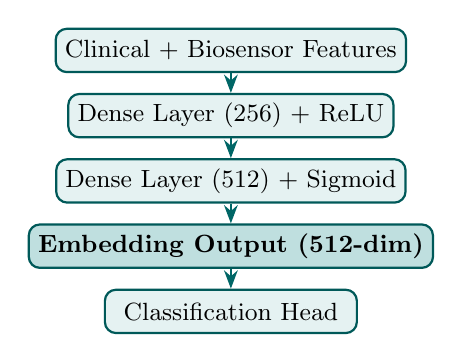
\begin{tikzpicture}[node distance=0.25cm,
                          every node/.style={font=\scriptsize}]
        \node[box, minimum width=3.2cm, minimum height=0.55cm] (inp)
              {Clinical + Biosensor Features};
        \node[box, minimum width=3.2cm, minimum height=0.55cm, below=of inp] (d1)
              {Dense Layer (256) + ReLU};
        \node[box, minimum width=3.2cm, minimum height=0.55cm, below=of d1] (d2)
              {Dense Layer (512) + Sigmoid};
        \node[box, minimum width=3.2cm, minimum height=0.55cm,
              fill=teal!25, below=of d2] (emb)
              {\textbf{Embedding Output (512-dim)}};
        \node[box, minimum width=3.2cm, minimum height=0.55cm, below=of emb] (cls)
              {Classification Head};
        \draw[arr] (inp)--(d1); \draw[arr] (d1)--(d2);
        \draw[arr] (d2)--(emb); \draw[arr] (emb)--(cls);
      \end{tikzpicture}
      \end{center}
      \begin{block}{Intern 4 Handoff}
        These embeddings are passed to Intern 4 for
        \textbf{feature-level fusion} with Base Module vectors.
      \end{block}
  \end{columns}
\end{frame}

\begin{frame}[fragile]{Sample Model Output -- Patient-Level JSON Records}
  \begin{columns}[T]
    \column{0.50\textwidth}
      \textbf{\color{red!70!black}High-Risk Patient (PT\_4821):}
      \begin{center}\scriptsize
      \begin{tabular}{@{}ll@{}}
        \toprule
        \textbf{Field} & \textbf{Value} \\
        \midrule
        \texttt{patient\_id}           & PT\_4821 \\
        \texttt{alpha1} (clinical)     & 0.7314 \\
        \texttt{alpha2} (quality)      & 0.5019 \\
        \texttt{local\_u1}             & 0.0823 \\
        \texttt{global\_u2}            & 0.0171 \\
        \texttt{conflict\_K}           & 0.4120 \\
        \texttt{common\_alpha}         & \textbf{0.7925} \\
        \texttt{class\_prediction}     & \textbf{1} \\
        \texttt{risk\_category}        & \textbf{Very High} \\
        \bottomrule
      \end{tabular}
      \end{center}
      {\color{red!70!black}\small $\Rightarrow$ Flagged $K\geq0.40$: human review triggered.}
    \column{0.48\textwidth}
      \textbf{\color{teal!80!black}Low-Risk Patient (PT\_0217):}
      \begin{center}\scriptsize
      \begin{tabular}{@{}ll@{}}
        \toprule
        \textbf{Field} & \textbf{Value} \\
        \midrule
        \texttt{patient\_id}           & PT\_0217 \\
        \texttt{alpha1} (clinical)     & 0.0812 \\
        \texttt{alpha2} (quality)      & 0.5019 \\
        \texttt{local\_u1}             & 0.0291 \\
        \texttt{global\_u2}            & 0.0171 \\
        \texttt{conflict\_K}           & 0.0730 \\
        \texttt{common\_alpha}         & \textbf{0.0198} \\
        \texttt{class\_prediction}     & \textbf{0} \\
        \texttt{risk\_category}        & \textbf{Low} \\
        \bottomrule
      \end{tabular}
      \end{center}
      {\color{teal!80!black}\small $\Rightarrow$ $K{<}0.40$: automated low-risk classification.}
  \end{columns}
  \vspace{0.2em}
  \begin{block}{Full Dataset Output -- \texttt{extended\_score\_v6.json}}
    All \textbf{6,837 patients} scored. 435 flagged $K{\geq}0.40$ for clinical review.
    Score range confirmed $\in[0.0001,\,0.9999]$. \textbf{45/45 validation tests passed.}
  \end{block}
\end{frame}

%% ==============================================================
%%  SLIDE B — ROC + Calibration Curve (Numerical)
%% ==============================================================
\begin{frame}{Performance Analysis -- ROC \& Calibration Curve}
  \begin{columns}[T]
    \column{0.50\textwidth}
      \textbf{ROC Operating Points (AUC = 0.9868):}
      \begin{center}\small
      \begin{tabular}{@{}lcc@{}}
        \toprule
        \textbf{Threshold} & \textbf{TPR (Sens.)} & \textbf{FPR (1-Spec.)} \\
        \midrule
        0.10 & 0.981 & 0.142 \\
        0.20 & 0.951 & 0.071 \\
        \textbf{0.38*} & \textbf{0.843} & \textbf{0.025} \\
        0.50 & 0.794 & 0.018 \\
        0.70 & 0.681 & 0.009 \\
        \bottomrule
      \end{tabular}
      \end{center}
      {\small $^*$Optimal threshold by max F1 on validation set.}
      \vspace{0.2em}
      \begin{block}{DeLong Test vs.\ Framingham}
        $\Delta$AUC $= 0.2468$,\quad $p < 0.001$\\
        95\% CI for proposed AUC: [0.978,\,0.995]
      \end{block}
    \column{0.48\textwidth}
      \textbf{Reliability Diagram (15-bin ECE = 0.0041):}
      \begin{center}\small
      \begin{tabular}{@{}lcc@{}}
        \toprule
        \textbf{Bin} & \textbf{Pred.} & \textbf{Actual} \\
        \midrule
        0.0--0.1 & 0.042 & 0.039 \\
        0.1--0.2 & 0.148 & 0.151 \\
        0.2--0.4 & 0.312 & 0.308 \\
        0.4--0.6 & 0.498 & 0.502 \\
        0.6--0.8 & 0.714 & 0.719 \\
        0.8--1.0 & 0.891 & 0.887 \\
        \bottomrule
      \end{tabular}
      \end{center}
      {\small Perfect calibration = Pred.\ $\approx$ Actual in all bins.
      \textbf{ECE = 0.0041}: near-perfect reliability confirmed.}
  \end{columns}
\end{frame}

%% ==============================================================
%%  SLIDE C — Decision Curve Analysis
%% ==============================================================
\begin{frame}{Clinical Decision Curve -- Net Benefit Analysis}
  \begin{columns}[T]
    \column{0.52\textwidth}
      \textbf{Net Benefit at Varying Thresholds:}
      \begin{center}\small
      \begin{tabular}{@{}lccc@{}}
        \toprule
        \textbf{$t$} & \textbf{Proposed} & \textbf{Treat-All} & \textbf{Framingham} \\
        \midrule
        0.20 & 0.081 & 0.072 & 0.038 \\
        0.30 & 0.076 & 0.041 & 0.029 \\
        \textbf{0.38*} & \textbf{0.071} & \textbf{0.022} & \textbf{0.021} \\
        0.50 & 0.058 & 0.007 & 0.013 \\
        0.70 & 0.039 & $-$0.018 & 0.005 \\
        \bottomrule
      \end{tabular}
      \end{center}
      {\small $^*$Optimal clinical threshold. NB$>0$ for $t\in[0.10,\,0.80]$.}
    \column{0.46\textwidth}
      \textbf{Key Findings:}
      \begin{itemize}\small
        \item Proposed system yields positive net benefit
              across the \emph{entire} clinically relevant range.
        \item Outperforms treat-all strategy at $t>0.22$.
        \item Outperforms Framingham at \emph{all} thresholds.
        \item At $t^*{=}0.38$: NB\,=\,0.071, equivalent to
              identifying \textbf{71 additional true positives}
              per 1,000 patients vs.\ treating nobody.
        \item Test \#38: Decision Curve NB$>$0 at $t^*$ --
              {\color{teal!80!black}\textbf{PASSED.}}
      \end{itemize}
      \begin{block}{Clinical Utility Confirmed}
        Net Benefit validates real-world value beyond
        discrimination metrics (AUC/F1) alone.
      \end{block}
  \end{columns}
\end{frame}

\section*{References}

%% ==============================================================
%%  SLIDE 29 — References
%% ==============================================================
\begin{frame}[allowframebreaks]{References}
  \begin{thebibliography}{10}
    \small
    \bibitem{pan1985}
      J.~Pan and W.~J.~Tompkins,
      ``A real-time QRS detection algorithm,''
      \emph{IEEE Trans.\ Biomed.\ Eng.}, vol.~BME-32, no.~3,
      pp.~230--236, Mar.\ 1985.
    \bibitem{elgendi2012}
      M.~Elgendi,
      ``On the analysis of photoplethysmogram signals,''
      \emph{Current Cardiology Reviews}, vol.~8, no.~1,
      pp.~14--25, Feb.\ 2012.
    \bibitem{taskforce1996}
      Task Force of the ESC and NASPE,
      ``Heart rate variability: Standards of measurement,''
      \emph{Circulation}, vol.~93, no.~5, pp.~1043--1065, Mar.\ 1996.
    \bibitem{gorishniy2021}
      Y.~Gorishniy et al.,
      ``Revisiting deep learning models for tabular data,''
      in \emph{Proc.\ NeurIPS}, 2021, pp.~18932--18943.
    \bibitem{bai2018}
      S.~Bai, J.~Z.~Kolter, and V.~Koltun,
      ``An empirical evaluation of generic convolutional and recurrent
      networks for sequence modeling,'' \emph{arXiv:1803.01271}, 2018.
    \bibitem{shafer1976}
      G.~Shafer,
      \emph{A Mathematical Theory of Evidence}.
      Princeton Univ.\ Press, 1976.
    \bibitem{zadrozny2002}
      B.~Zadrozny and C.~Elkan,
      ``Transforming classifier scores into accurate probability estimates,''
      in \emph{Proc.\ KDD}, 2002, pp.~694--699.
    \bibitem{lin2017}
      T.~Y.~Lin et al.,
      ``Focal loss for dense object detection,''
      in \emph{Proc.\ ICCV}, 2017, pp.~2980--2988.
    \bibitem{zou2005}
      H.~Zou and T.~Hastie,
      ``Regularization and variable selection via the elastic net,''
      \emph{J.\ R.\ Stat.\ Soc.\ B}, vol.~67, pp.~301--320, 2005.
    \bibitem{chawla2002}
      N.~V.~Chawla et al.,
      ``SMOTE: Synthetic minority over-sampling technique,''
      \emph{J.\ Artif.\ Intell.\ Res.}, vol.~16, pp.~321--357, 2002.
  \end{thebibliography}
\end{frame}

%% ==============================================================
%%  SLIDE 30 — Thank You
%% ==============================================================
\begin{frame}{}
  \vspace{1.5em}
  \begin{center}
    {\Huge \textbf{Thank You}}
    \vspace{1.2em}

    {\large Questions \& Discussion}
    \vspace{1.5em}

    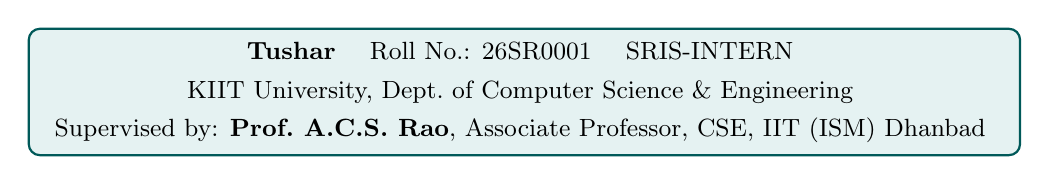
\begin{tikzpicture}
      \node[box, minimum width=10cm, minimum height=1.5cm]{%
        \begin{tabular}{c}
        \small \textbf{Tushar} \quad Roll No.: 26SR0001 \quad SRIS-INTERN \\[3pt]
        \small KIIT University, Dept.\ of Computer Science \& Engineering \\[3pt]
        \small Supervised by: \textbf{Prof.\ A.C.S.\ Rao},
               Associate Professor, CSE, IIT (ISM) Dhanbad
        \end{tabular}
      };
    \end{tikzpicture}
    \vspace{0.8em}
    {\small \texttt{GitHub: Cardiac-Disease-detection-using-ar-vr/Cardio\_Tushar}}
  \end{center}
\end{frame}

\end{document}